\pgfplotsset{width=7cm,compat=1.16}
\usepgfplotslibrary{polar}

\begin{document}
% eg, ie, etc, wrt, viz newcommands
\newcommand{\eg}{{\it e.g.\@}} % \@ for normal spacing after. use: \eg\/ or \eg,
\newcommand{\ie}{{\it i.e.\@}} 
\newcommand{\wrt}{{\it wrt}}
\newcommand{\viz}{{\it viz.\@}}
\newcommand{\vs}{{\it vs.\@}}
\newcommand{\aka}{{\it aka}}
\newcommand{\apriori}{{\it a priori}}
\newcommand{\etc}{\textit{etc.\@}}    
\newcommand{\bank}{../../questionBank}                                            
% etc defined so that there is only a single period after it if it is followed 
% by a period
% see: http://en.wikibooks.org/wiki/TeX/def                                      
% see: http://www.tug.org/pipermail/texhax/2004-July/002449.html                 
% see: http://en.wikibooks.org/wiki/TeX/if                                       
%\ifx \etc \undefined                                                             
%  %\def\myarg{#1}                                                                
%  %\def\myfullstop{.}                                                            
%  %\def\etc{#1}{\textit{etc} arg is ``\myarg'' \ifx\myarg\myfullstop\then.\else.#1\fi\/}
%  \def\etc#1{\textit{etc}\if#1..\else.#1\fi}                                     
%\fi                                                                              
%                        

% this should be moved to a new newcommands file
\newcommand{\ignore}[1]{}


\qns{Complex Numbers}

A complex number, $z$, is composed of a real part and imaginary part.
If $z = a + bj$, then $\mathfrak{Re}(z) = a$ (the real portion equals a), and $\mathfrak{Im}(z) = b$ (the imaginary portion equals b).
Complex numbers can be expressed in two ways:

\begin{center}
Rectangular Form: $z = a + bj$ \hspace{1em} Polar Form: $z = re^{j\theta}$
\end{center}

In polar form, $r$ represents the magnitude and $\theta$ represents the angle of the complex number with respect to the origin of the complex plane.
Rectangular form makes adding and subtracting complex numbers easier; whereas, polar form makes multiplying and dividing numbers easier.
Some handy equations to switch between forms include:

\begin{center}

\begin{tabular}{ c c c }
 $\tan(\theta) = \frac{b}{a}$ & $r = |z| = \sqrt{a^2 + b^2}$ \\ \\
 $\sin(\theta) = \frac{b}{|z|}$ & $\cos(\theta) = \frac{a}{|z|}$ \\  \\
\end{tabular}

\end{center}

\begin{enumerate}

\qitem Use Euler's formulas to convert between the two forms.

\begin{enumerate}
\qitem Convert 10 + 12j to polar form.

\sol{
$z = a + bj$. We can go from rectangular form to polar form by using the equation $z = |z|e^{j\theta}$, where $|z| = \sqrt{a^2 + b^2}$ and $\theta = \angle z = \tan^{-1}(\frac{b}{a})$.
$$ z = 10 + 12j $$
$$ |z| = \sqrt{10^2 + 12^2} = \sqrt{244}$$
$$ \angle z = \tan^{-1}(\frac{12}{10})$$
$$ z = \sqrt{244}e^{j \, {\tan^{-1}(\frac{12}{10})}} \approx 15.620e^{0.876j}$$
}

\qitem Convert $22e^{23j}$ to rectangular form.

\sol{
Conversely, for $z = |z|e^{j\theta}$, we can go from polar form to rectangular form by using the equation $z = a + bj$, where $a = |z|\cos(\theta)$ and $b = |z|\sin(\theta)$. So, \\
$$ a = 22\cos(23) $$
$$ b = 22\sin(23) $$
$$ z = 22\cos(23) + 22j \sin(23) \approx -11.722 + -18.617j$$
}
\end{enumerate}


\qitem Plot the following on a polar grid:
\begin{enumerate}

\qitem {2}

\sol {
\newline
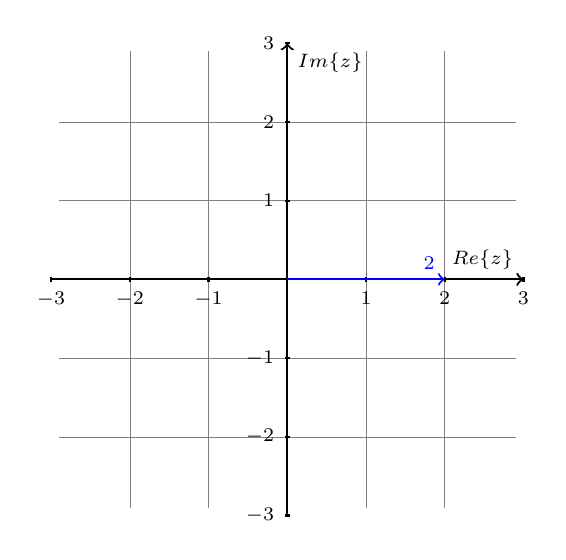
\begin{tikzpicture}
    \begin{scope}[thick,font=\scriptsize]
    \draw[step=1cm,gray,very thin] (-2.9,-2.9) grid (2.9,2.9);
    \draw [->] (-3,0) -- (3,0) node [above left]  {$Re\{z\}$};
    \draw [->] (0,-3) -- (0,3) node [below right] {$Im\{z\}$};
    
    \foreach \x in {-3, -2, -1, 1, 2, 3}
       \draw (\x cm,1pt) -- (\x cm,-1pt) node[anchor=north] {$\x$};
    \foreach \y in {-3, -2, -1, 1, 2, 3}
        \draw (1pt,\y cm) -- (-1pt,\y cm) node[anchor=east] {$\y$};
    
    
    \draw [line width=0.25mm, blue, ->] (0,0) -- (2,0) node [above left] {2};
    \end{scope}
\end{tikzpicture}
}

\qitem {2j}

\sol {
\newline
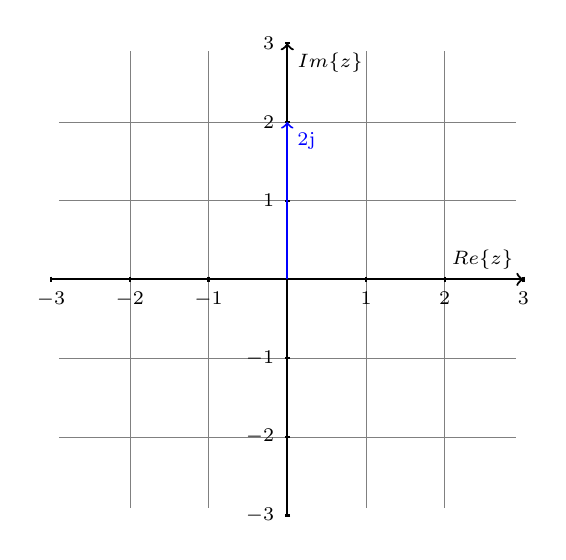
\begin{tikzpicture}
    \begin{scope}[thick,font=\scriptsize]
    \draw[step=1cm,gray,very thin] (-2.9,-2.9) grid (2.9,2.9);
    \draw [->] (-3,0) -- (3,0) node [above left]  {$Re\{z\}$};
    \draw [->] (0,-3) -- (0,3) node [below right] {$Im\{z\}$};
    
    \foreach \x in {-3, -2, -1, 1, 2, 3}
       \draw (\x cm,1pt) -- (\x cm,-1pt) node[anchor=north] {$\x$};
    \foreach \y in {-3, -2, -1, 1, 2, 3}
        \draw (1pt,\y cm) -- (-1pt,\y cm) node[anchor=east] {$\y$};
    
    
    \draw [line width=0.25mm, blue, ->] (0,0) -- (0,2) node [below right] {2j};
    \end{scope}
\end{tikzpicture}

}

\qitem {2 + 2j}

\sol {
\newline
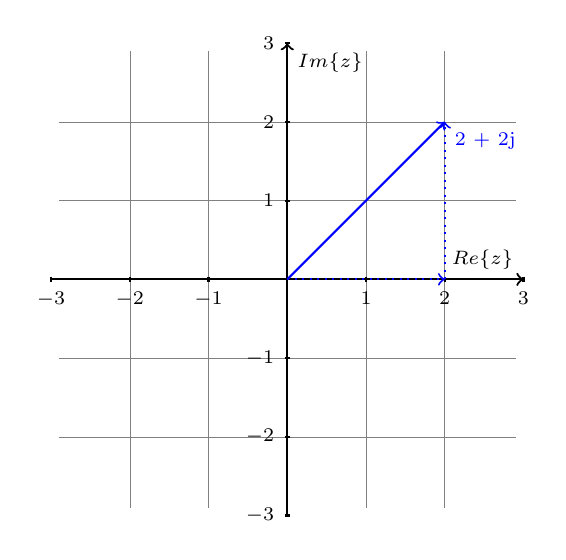
\begin{tikzpicture}
    \begin{scope}[thick,font=\scriptsize]
    \draw[step=1cm,gray,very thin] (-2.9,-2.9) grid (2.9,2.9);
    \draw [->] (-3,0) -- (3,0) node [above left]  {$Re\{z\}$};
    \draw [->] (0,-3) -- (0,3) node [below right] {$Im\{z\}$};
    
    \foreach \x in {-3, -2, -1, 1, 2, 3}
       \draw (\x cm,1pt) -- (\x cm,-1pt) node[anchor=north] {$\x$};
    \foreach \y in {-3, -2, -1, 1, 2, 3}
        \draw (1pt,\y cm) -- (-1pt,\y cm) node[anchor=east] {$\y$};
    
    
    \draw [line width=0.25mm, blue, ->] (0,0) -- (2,2) node [below right] {2 + 2j};
    \draw [dotted, line width=0.25mm, blue, ->] (0,0) -- (2,0) node [below right] {};
    \draw [dotted, line width=0.25mm, blue, ->] (2,0) -- (2,2) node [below right] {};
    \end{scope}

\end{tikzpicture}

}

\end{enumerate}

\qitem Calculate the magnitude and phase of the following:
\begin{enumerate}

\qitem {2}

\sol {
$$z = 2 + 0j.$$
$$|z| = \sqrt{2^2 + 0^2} = 2.$$
$$\angle z = \angle 2 = 0 \, \text{rad}. $$
}

\qitem $\frac{2}{2j}$

\sol {
$$ z = \frac{2}{2j} = (\frac{1}{j})(\frac{j}{j}) = \frac{j}{j^2} = -j = 0 - 1j.$$
$$|z| = \sqrt{0^2 + (-1)^2} = 1.$$
$$\angle z = \angle -j = \frac{3\pi}{2} \, \text{rad}.$$
}

\qitem $\frac{3j}{5}$

\sol {
$$z = 0 + \frac{3}{5}j.$$
$$|z| = \sqrt{0^2 + \frac{3}{5}^2} = \frac{3}{5}.$$ 
$$\angle z = \angle \frac{3}{5}j = \frac{\pi}{2} \, \text{rad}.$$
}

\qitem $\frac{1+2j}{9+7j}$

\sol {
$$z = \frac{1+2j}{9+7j} = \frac{z_a}{z_b}.$$
$$|z| = \frac{|z_a|}{|z_b|} = \frac{\sqrt{1^2 + 2^2}}{\sqrt{9^2 + 7^2}} = \frac{\sqrt{5}}{\sqrt{130}}. \approx 0.196.$$
$$\angle z = \angle z_a - \angle z_b = \tan^{-1}(\frac{2}{1}) - \tan^{-1}(\frac{7}{9}) = 1.107 + 0.661 \approx 1.768 \, \text{rad}.$$
}

\end{enumerate}


\qitem Prove algebraically that $\frac{1}{j} = -j$.

\sol{
The key is to multiply the left-hand side of the equation by $\frac{j}{j}$: \\
$$\frac{1}{j} = \frac{1 * j}{j * j} = \frac{j}{j^2}$$
$$= \frac{j}{-1} = -j$$
}

\end{enumerate}

A complex number, $z = a + bj$ has a complex conjugate, $\overline{z} = a - bj$.
Note that the sum of a complex number and its conjugate is always real, but the difference between a complex number and its conjugate is always imaginary.

\begin{enumerate}[resume]

\qitem Use a polar graph to show that the sum of any complex number and its conjugate is always real.

\sol{
For complex number $z = a + bj$, its conjugate is $\bar{z} = a - bj$. If we add these two together, we get $z + \bar{z} = a + bj + a - bj = 2a + 0j$. The imaginary components cancel out exactly, so the resulting sum is always entirely real. This is illustrated by the following graph for $z = 1 + 1j$ and $\bar{z} = 1 - 1j$:

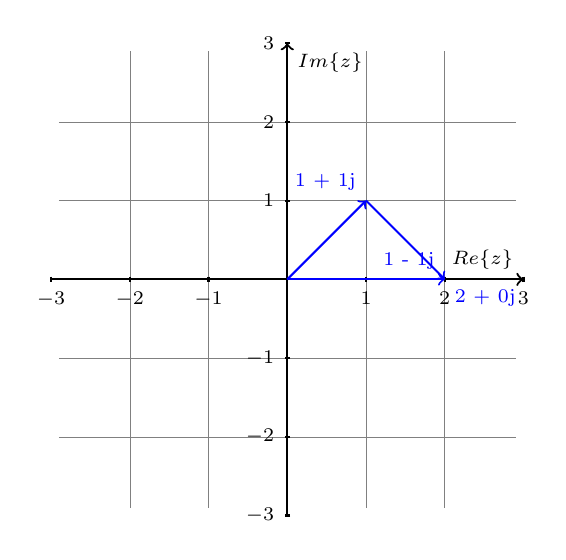
\begin{tikzpicture}
    \begin{scope}[thick,font=\scriptsize]
    \draw[step=1cm,gray,very thin] (-2.9,-2.9) grid (2.9,2.9);
    \draw [->] (-3,0) -- (3,0) node [above left]  {$Re\{z\}$};
    \draw [->] (0,-3) -- (0,3) node [below right] {$Im\{z\}$};
    
    \foreach \x in {-3, -2, -1, 1, 2, 3}
       \draw (\x cm,1pt) -- (\x cm,-1pt) node[anchor=north] {$\x$};
    \foreach \y in {-3, -2, -1, 1, 2, 3}
        \draw (1pt,\y cm) -- (-1pt,\y cm) node[anchor=east] {$\y$};
    
    
    \draw [line width=0.25mm, blue, ->] (0,0) -- (1,1) node [above left] {1 + 1j};
    \draw [line width=0.25mm, blue, ->] (1,1) -- (2,0) node [above left] {1 - 1j};
    \draw [line width=0.25mm, blue, ->] (0,0) -- (2,0) node [below right] {2 + 0j};
    \end{scope}
\end{tikzpicture}

}

\qitem Recall that Euler's Formula states that $e^{j\theta} = \cos(\theta) + j\sin(\theta)$.
Using Euler's identity, show that $\cos(\theta) = \frac{1}{2}(e^{j\theta} + e^{-j\theta})$.

\sol{

  $$e^{j\theta} = \cos(\theta) + j\sin(\theta)$$

  Note that $e^{j\theta}$ has the complex conjugate $e^{-j\theta}$, which means:

  $$e^{-j\theta} = \cos(\theta) - j\sin(\theta)$$
  $$e^{j\theta} +  e^{-j\theta} = \cos(\theta) + j\sin(\theta) + \cos(\theta) - j\sin(theta)$$
  $$e^{j\theta} +  e^{-j\theta} = 2\cos(\theta)$$
  $$cos(\theta) = \frac{1}{2}(e^{j\theta} +  e^{-j\theta})$$

}

\end{enumerate}


\end{document}